All discussion so far involved either simulated samples, Belle~II data samples with \BtoXsgamma events negligible,
or with the signal region ($\EB\in(1.8,2.7)~\gev$) hidden.
After preparing the analysis on simulation, performing extensive validation and evaluating systematic uncertainties, 
the signal region is ready to be unblinded, as it was shown that no significant biases are expected.
This section presents the results of the analysis.

\subsection{\texorpdfstring{\Mbc}{Mbc} fit results}\label{sec:mbc_fit_results}

Following the \Mbc fitting strategy described in \Cref{sec:fitting_setup} and the model in \Cref{tab:fitting_init_params_updated},
the fits on the signal region of Belle~II data are performed.
They are shown in \Cref{fig:data_fits_signal}.
Together with fits in \Cref{fig:sideband_data_fit}, it gives all the fits for the defined \EB intervals in \Cref{sec:binning}.
The extracted $\mathcal{N}_{\mathrm{CB}}$ are shown in the top right corner of each figure.
\begin{figure}[htbp!]
    \centering
    \subcaptionbox{\label{fig:data_fit_1p8_2p0}}{
        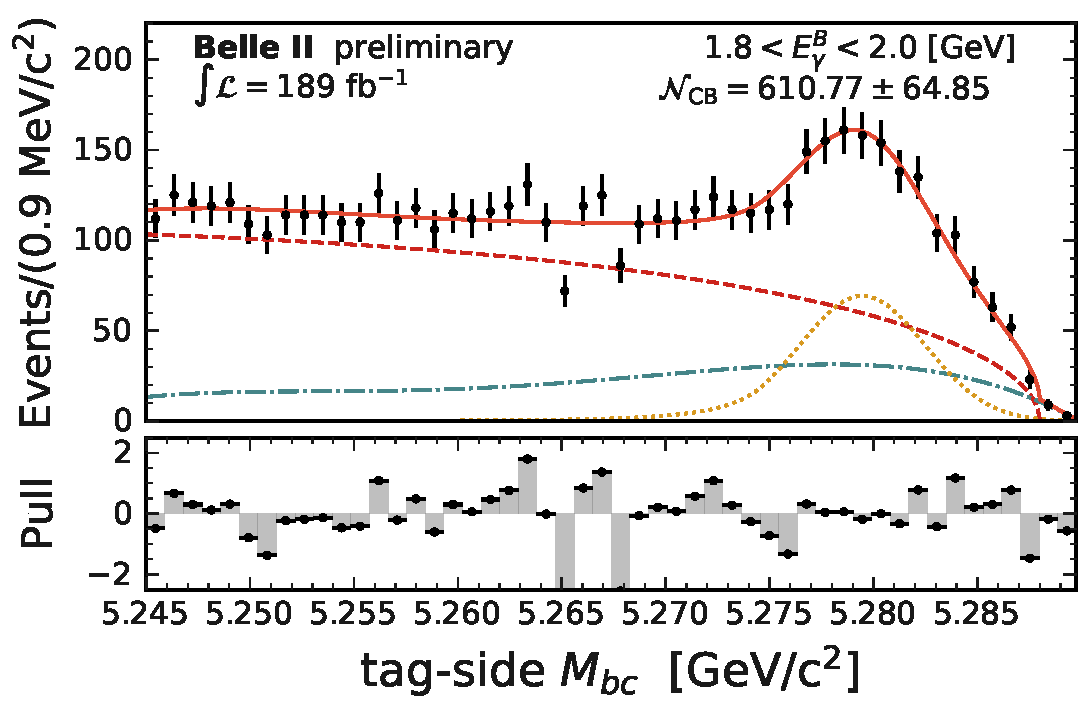
\includegraphics[width=0.3\textwidth]{figures/final_results/data_fits/DATA_MbcFit_1p8to2p0ppdf.pdf}
    }
    \subcaptionbox{\label{fig:data_fit_2p0_2p1}}{
        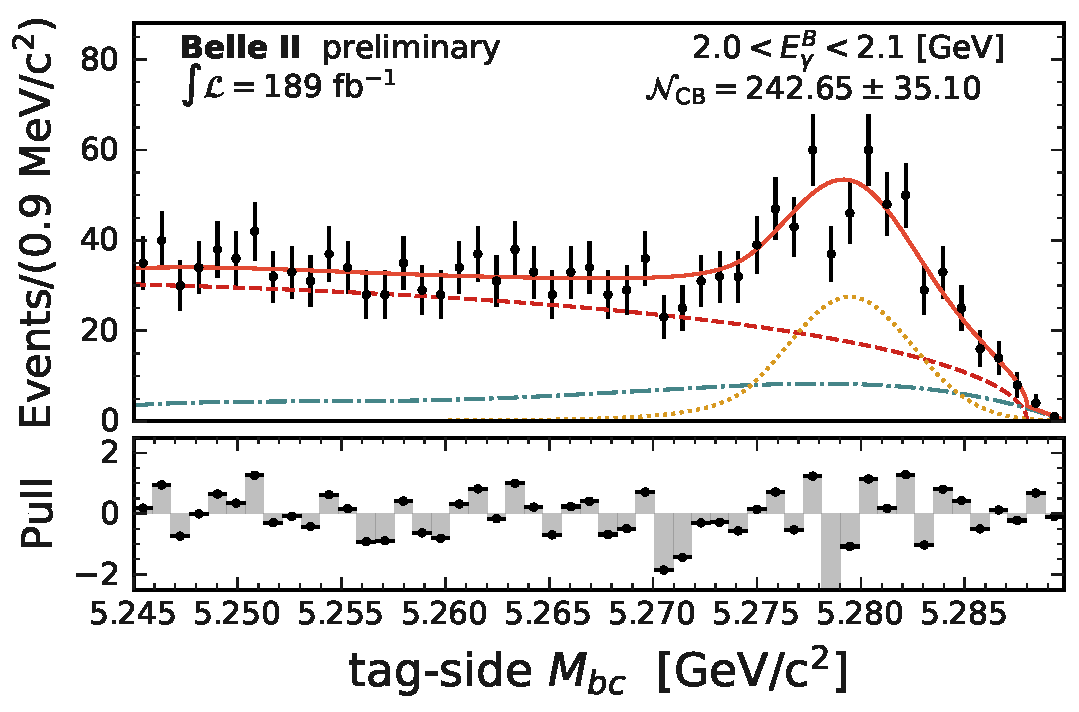
\includegraphics[width=0.3\textwidth]{figures/final_results/data_fits/DATA_MbcFit_2p0to2p1ppdf.pdf}
    }
    \subcaptionbox{\label{fig:data_fit_2p1_2p2}}{
        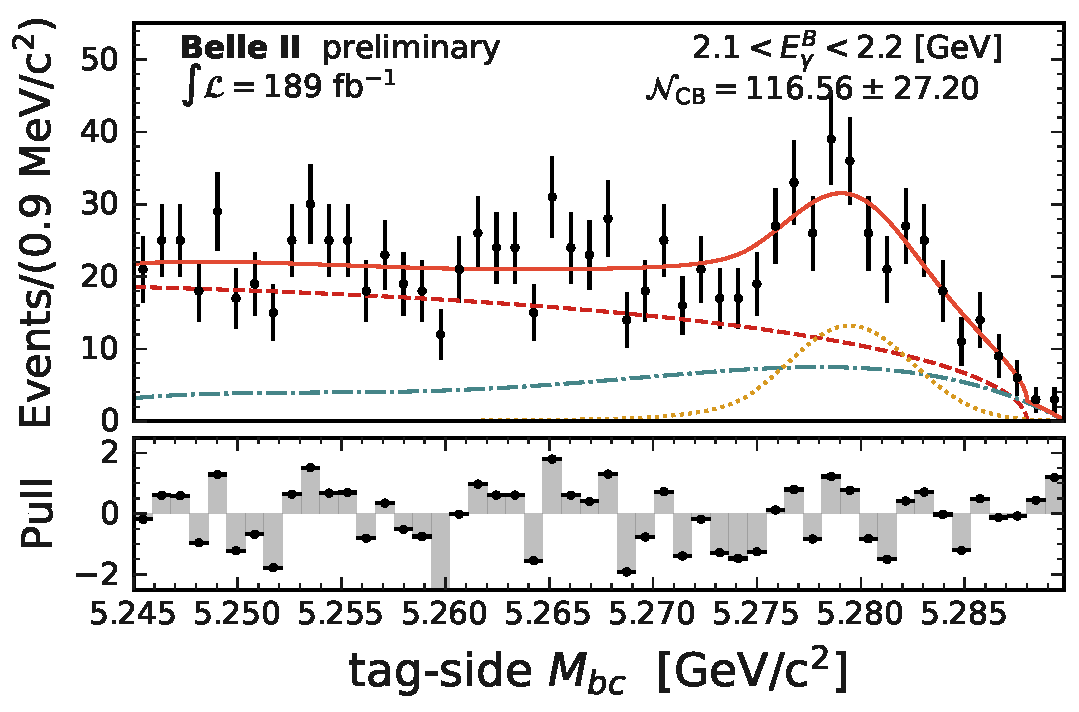
\includegraphics[width=0.3\textwidth]{figures/final_results/data_fits/DATA_MbcFit_2p1to2p2ppdf.pdf}
    }
    \subcaptionbox{\label{fig:data_fit_2p2_2p3}}{
        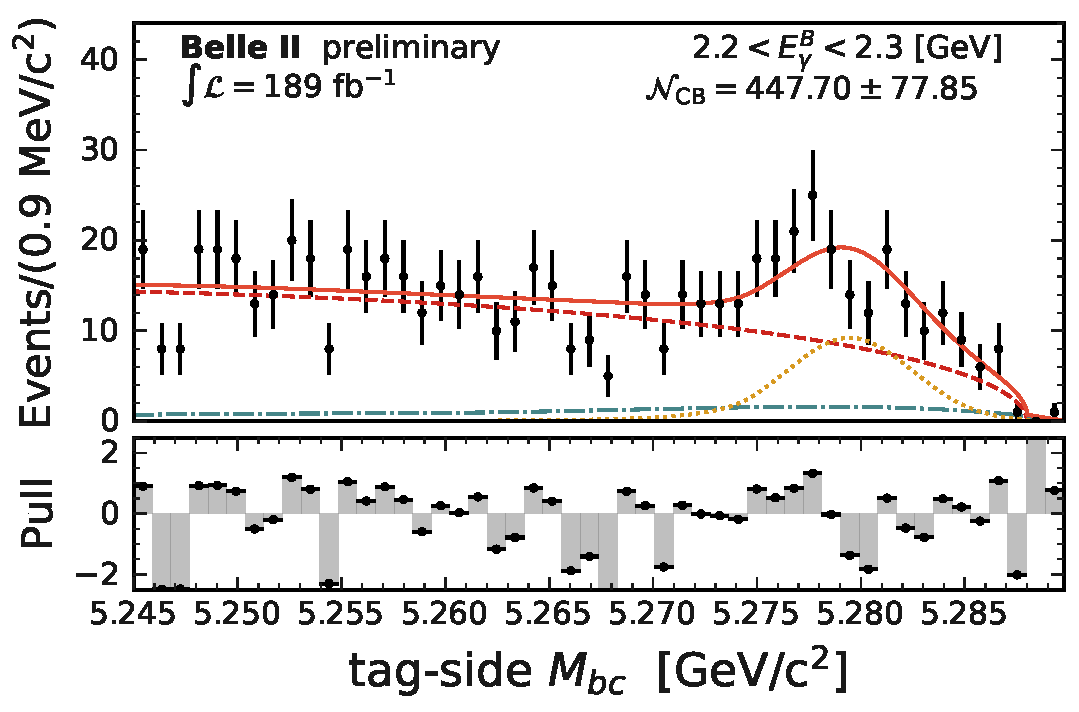
\includegraphics[width=0.3\textwidth]{figures/final_results/data_fits/DATA_MbcFit_2p2to2p3ppdf.pdf}        
    }
    \subcaptionbox{\label{fig:data_fit_2p3_2p4}}{
        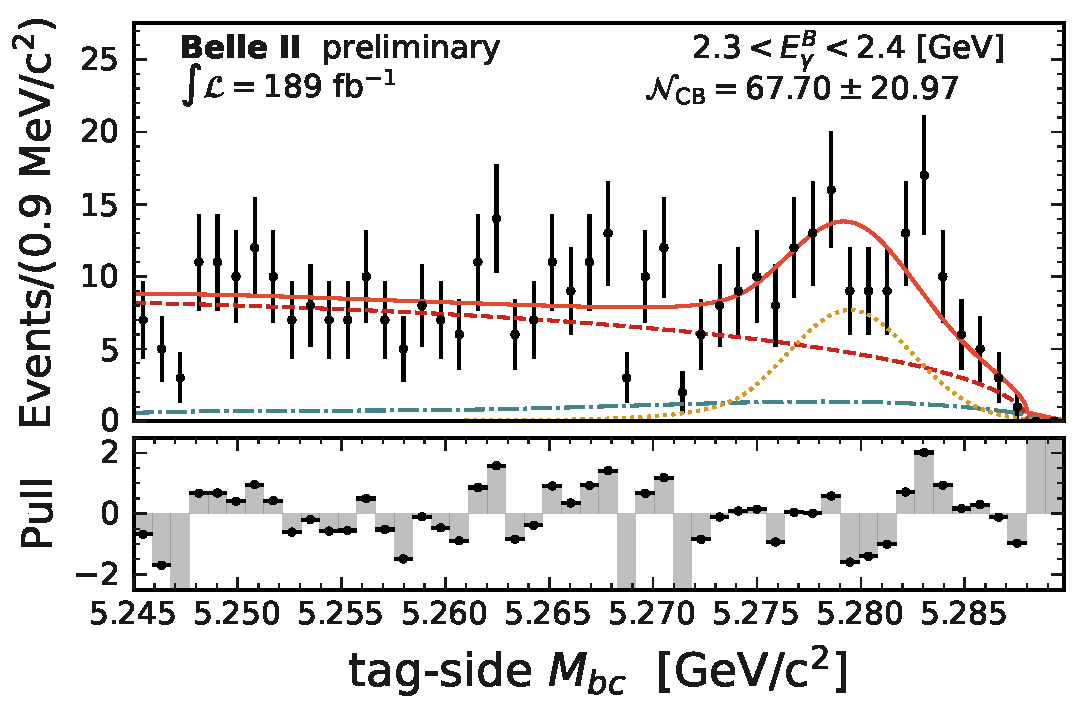
\includegraphics[width=0.3\textwidth]{figures/final_results/data_fits/DATA_MbcFit_2p3to2p4ppdf.pdf}
    }
    \subcaptionbox{\label{fig:data_fit_2p4_2p5}}{
        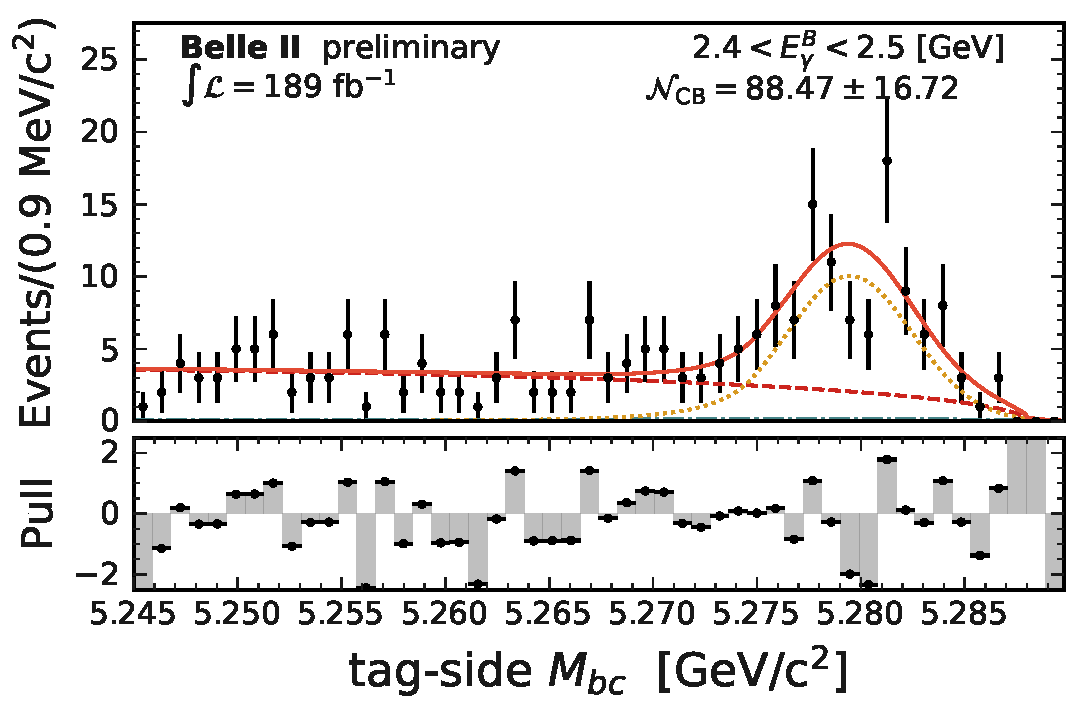
\includegraphics[width=0.3\textwidth]{figures/final_results/data_fits/DATA_MbcFit_2p4to2p5ppdf.pdf}
    }
    \subcaptionbox{\label{fig:data_fit_2p5_2p6}}{
        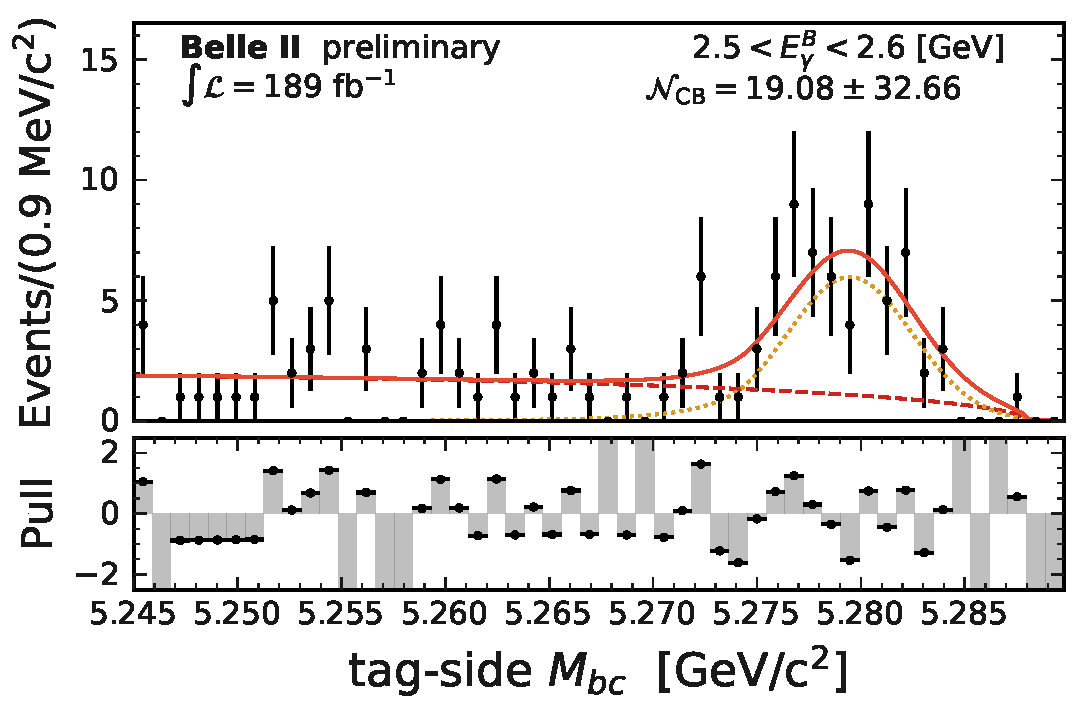
\includegraphics[width=0.3\textwidth]{figures/final_results/data_fits/DATA_MbcFit_2p5to2p6ppdf.pdf}
    }
    \subcaptionbox{\label{fig:data_fit_2p6_2p7}}{
        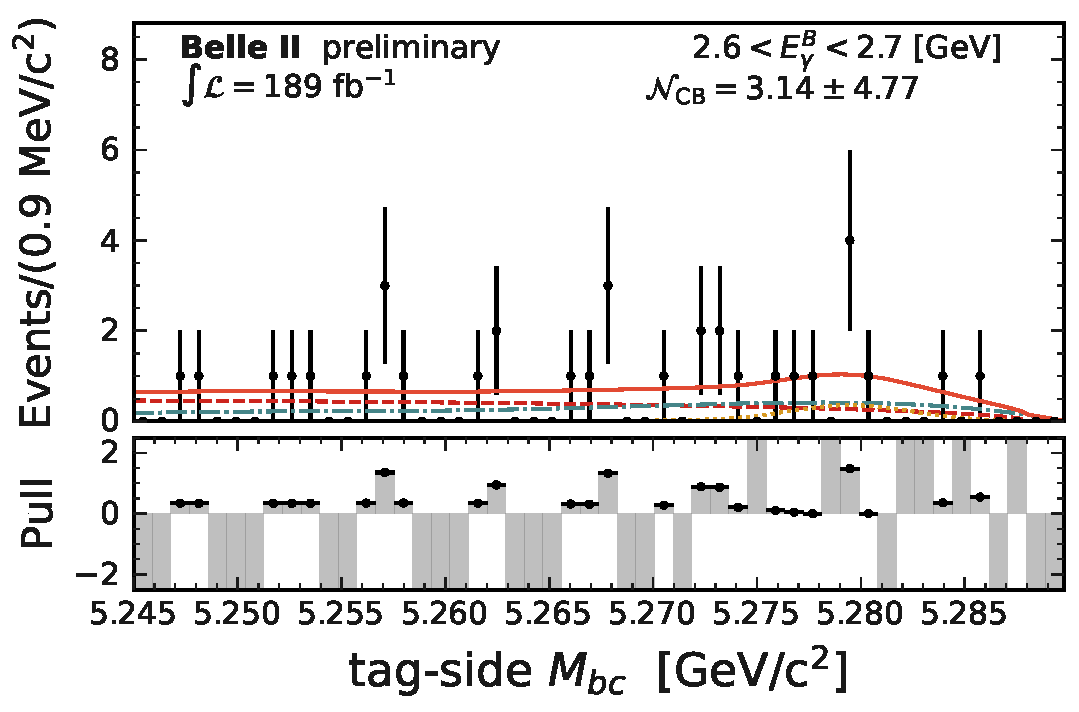
\includegraphics[width=0.3\textwidth]{figures/final_results/data_fits/DATA_MbcFit_2p6to2p7ppdf.pdf}        
    }
    \caption{\label{fig:data_fits_signal}
    The \EB signal region fits on the Belle~II data, based on the fitting model in \Cref{tab:fitting_init_params_updated}.
    The fits are performed as unbinned negative log-likelihood fits.
    The different \EB intervals are shown in the top right corner of each Figure, 
    together with the extracted good tag-\B meson yield, $\mathcal{N}_{\mathrm{CB}}$, which in this case corresponds to remaining good tag-\B backgrounds including \BtoXsgamma and other \BB decay channels.
    The fits outside of the signal region are provided in \Cref{fig:sideband_data_fit}.
    }
\end{figure}

The fit results on Belle~II simulation, with all \BtoXsgamma events removed, are shown in \Cref{fig:nosignal_fits_signal}.
The extracted number of \BB background events is shown in the top right corner of each figure.
These values are corrected, scaled, and are equal to the ones listed in \Cref{tab:background_uncertainties}.
Together with fits in \Cref{fig:sideband_mc_fit}, it gives all the fits for the defined \EB intervals in \Cref{sec:binning}.
\begin{figure}[htbp!]
    \centering
    \subcaptionbox{\label{fig:nosignal_fit_1p8_2p0}}{
        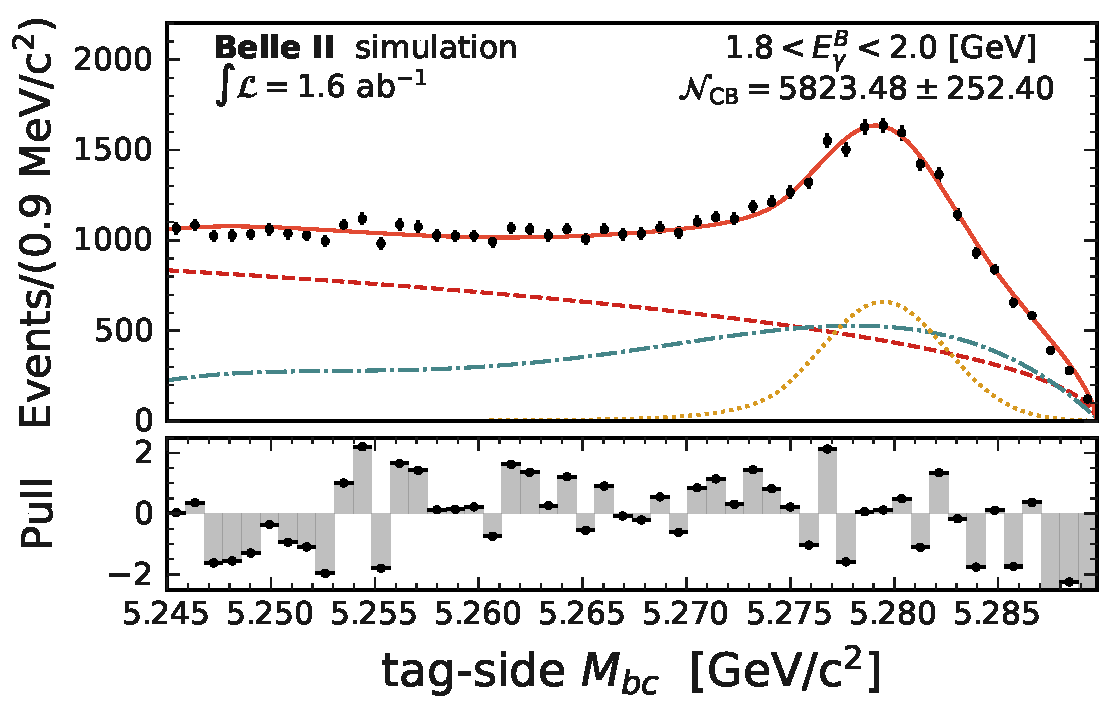
\includegraphics[width=0.3\textwidth]{figures/final_results/mc_fits/NOSIGNALMC_MbcFit_1p8to2p0ppdf.pdf}
    }
    \subcaptionbox{\label{fig:nosignal_fit_2p0_2p1}}{
        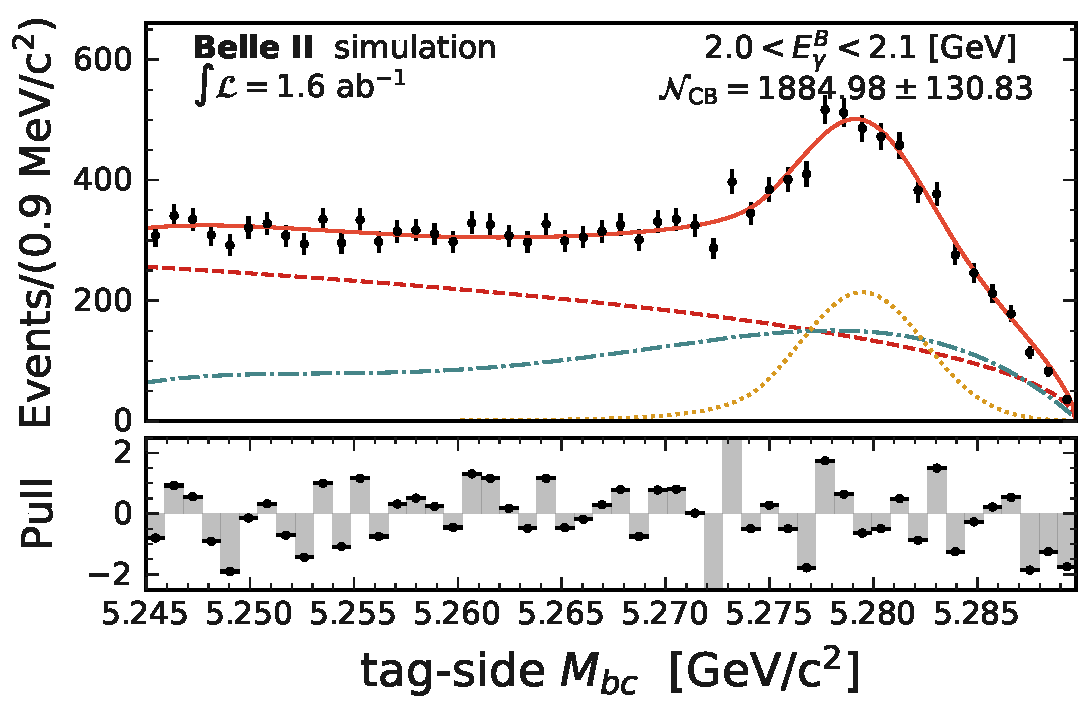
\includegraphics[width=0.3\textwidth]{figures/final_results/mc_fits/NOSIGNALMC_MbcFit_2p0to2p1ppdf.pdf}
    }
    \subcaptionbox{\label{fig:nosignal_fit_2p1_2p2}}{
        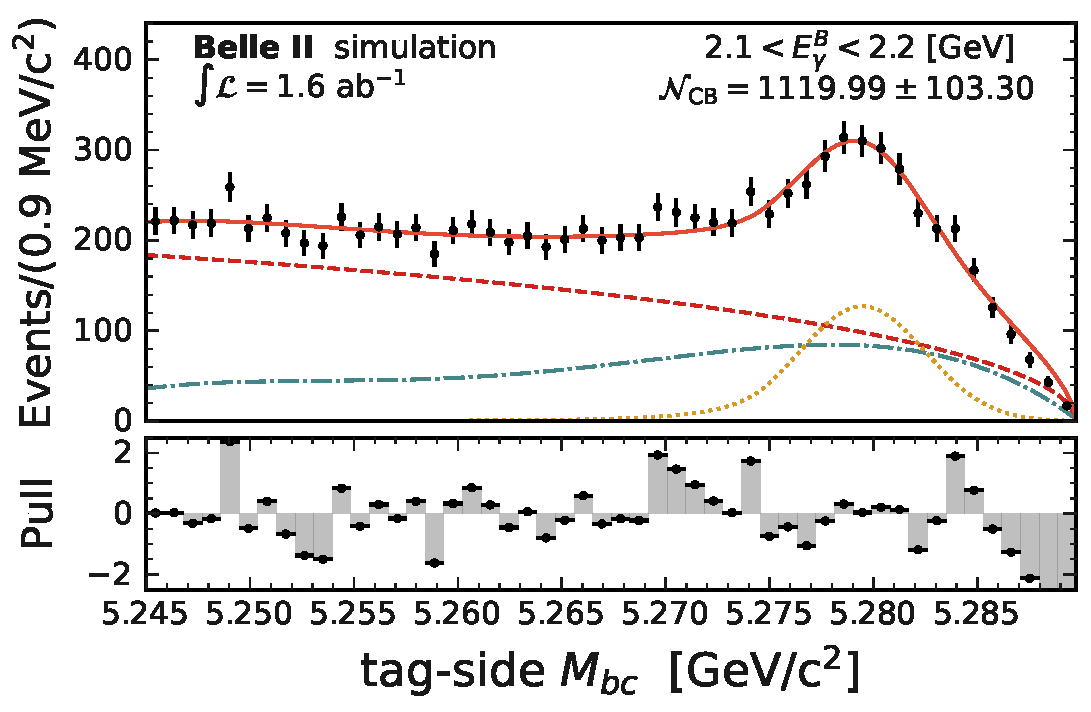
\includegraphics[width=0.3\textwidth]{figures/final_results/mc_fits/NOSIGNALMC_MbcFit_2p1to2p2ppdf.pdf}
    }
    \subcaptionbox{\label{fig:nosignal_fit_2p2_2p3}}{
        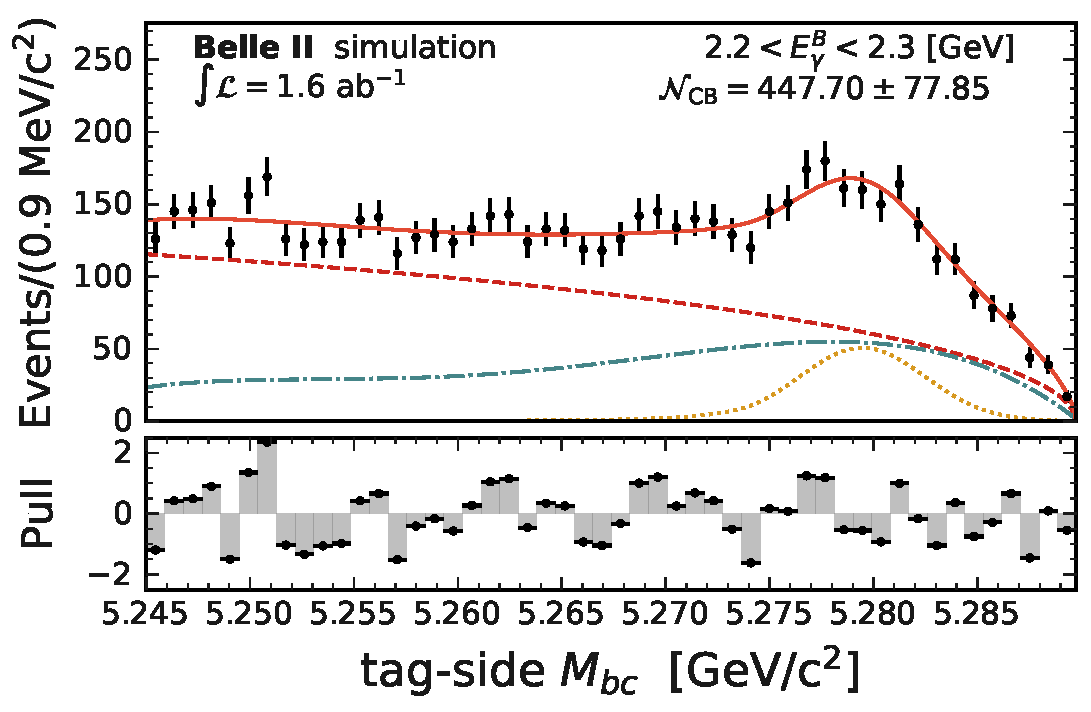
\includegraphics[width=0.3\textwidth]{figures/final_results/mc_fits/NOSIGNALMC_MbcFit_2p2to2p3ppdf.pdf}        
    }
    \subcaptionbox{\label{fig:nosignal_fit_2p3_2p4}}{
        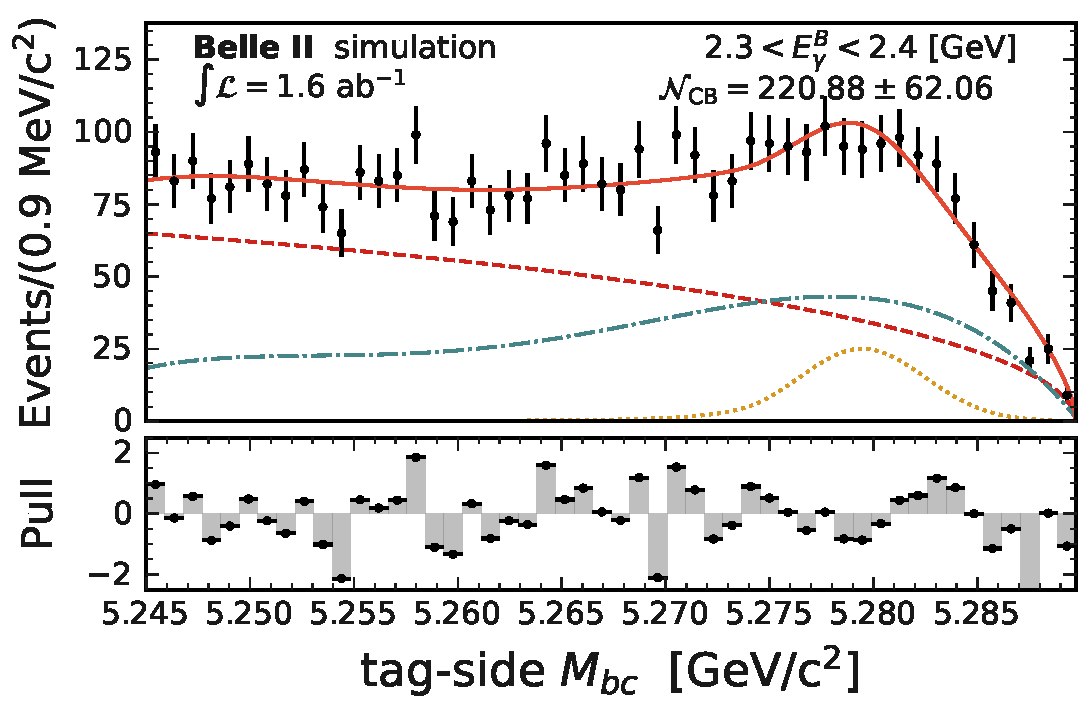
\includegraphics[width=0.3\textwidth]{figures/final_results/mc_fits/NOSIGNALMC_MbcFit_2p3to2p4ppdf.pdf}
    }
    \subcaptionbox{\label{fig:nosignal_fit_2p4_2p5}}{
        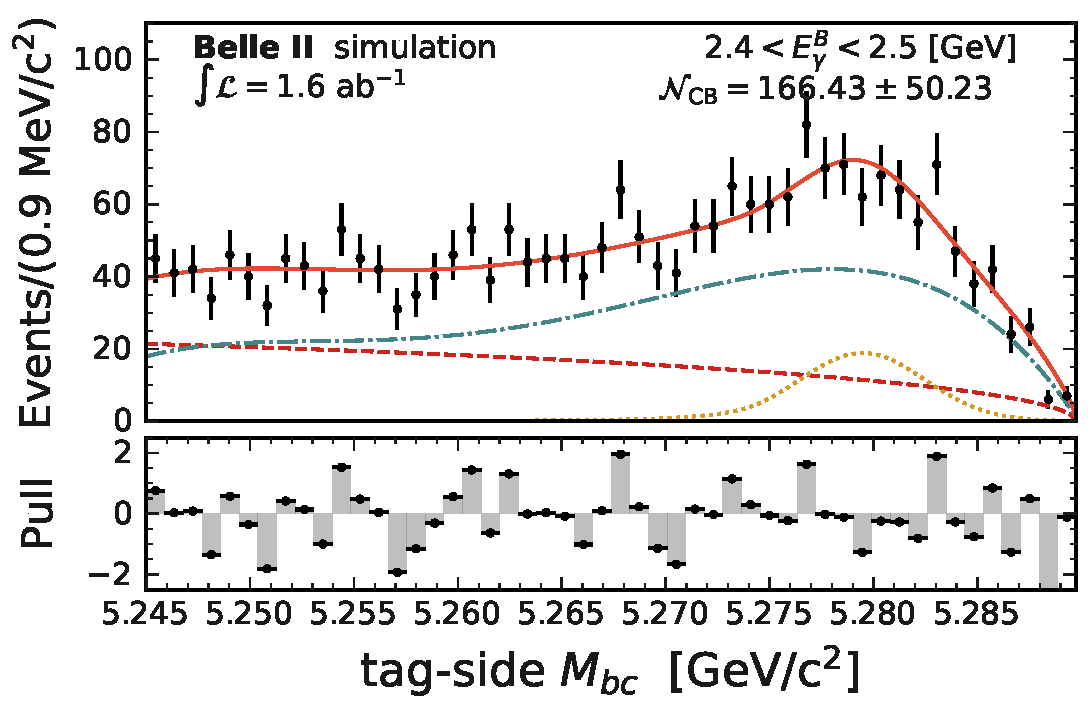
\includegraphics[width=0.3\textwidth]{figures/final_results/mc_fits/NOSIGNALMC_MbcFit_2p4to2p5ppdf.pdf}
    }
    \subcaptionbox{\label{fig:nosignal_fit_2p5_2p6}}{
        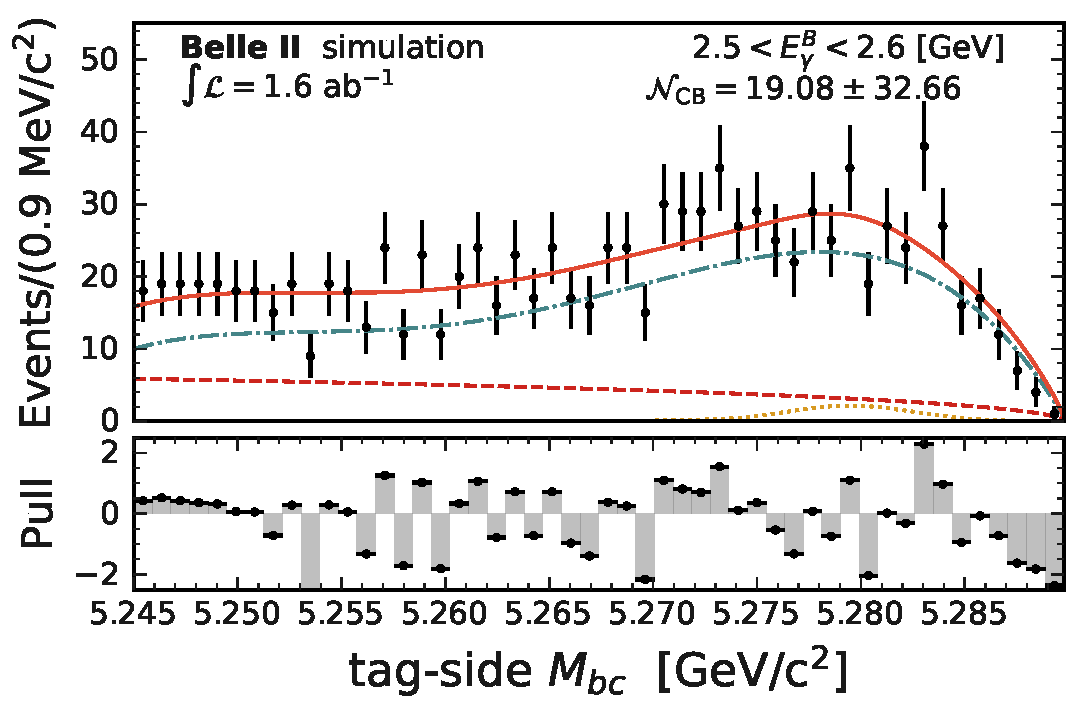
\includegraphics[width=0.3\textwidth]{figures/final_results/mc_fits/NOSIGNALMC_MbcFit_2p5to2p6ppdf.pdf}
    }
    \subcaptionbox{\label{fig:nosignal_fit_2p6_2p7}}{
        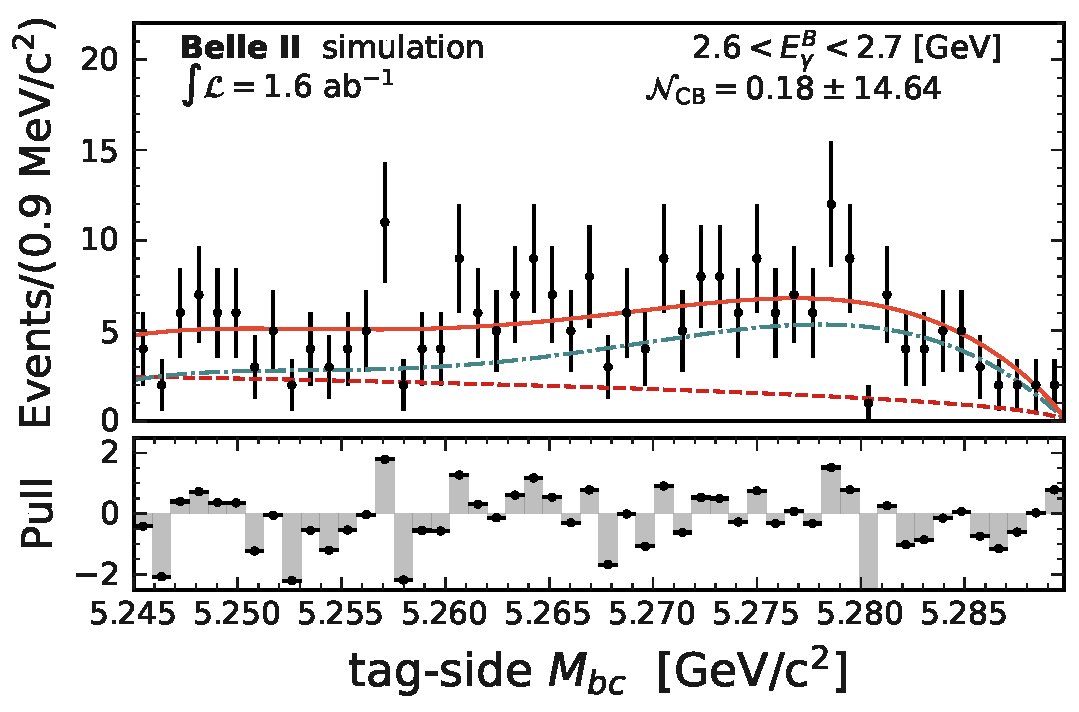
\includegraphics[width=0.3\textwidth]{figures/final_results/mc_fits/NOSIGNALMC_MbcFit_2p6to2p7ppdf.pdf}        
    }
    \caption{\label{fig:nosignal_fits_signal}
    The \EB signal region fits on the Belle~II simulation, where the \BtoXsdgamma events have been removed.
    The fitting model is summarised in \Cref{tab:fitting_init_params_updated}.
    The fits are performed as unbinned negative log-likelihood fits.
    The different \EB intervals are shown in the top right corner of each Figure, 
    together with the extracted good tag-\B meson yield, $\mathcal{N}_{\mathrm{CB}}$, which in this case corresponds only to non-\BtoXsdgamma events with good tag-\B mesons.
    The fits outside of the signal region are provided in \Cref{fig:sideband_data_fit}.
    }
\end{figure}

The number of good tag-\B events, evaluated from fits in Belle~II data (\Cref{fig:sideband_data_fit,fig:data_fits_signal}),
are summarised in \Cref{fig:final_fit_results}.
The figure also includes results from fots on Belle~II simulation with all \BtoXsgamma events removed (\Cref{fig:sideband_mc_fit,fig:nosignal_fits_signal}).
The latter provides the expectations of \BB backgrounds that remain in Belle~II data after the fit.
The simulation is corrected as discussed in \Cref{sec:corrections}, with appropriate uncertainties from \Cref{sec:systematic_uncertainty} included.
The \Cref{fig:final_fit_results_lin} shows the $\mathcal{N}_{\mathrm{CB}}$ in linear axis, which makes the comparison of low-\EB region easier. 
In this region, the number of signal events is expected to be much larger than any contribution from \BtoXsgamma events.
On the other hand, \Cref{fig:final_fit_results_log} shows the results in a logarithmic axis, which makes it evident that an excess over the remaining-\BB background is present.
This excess in data is evidence of \BtoXsdgamma events.

\begin{figure}[htbp!]
    \centering
    \subcaptionbox{\label{fig:final_fit_results_lin}}{
        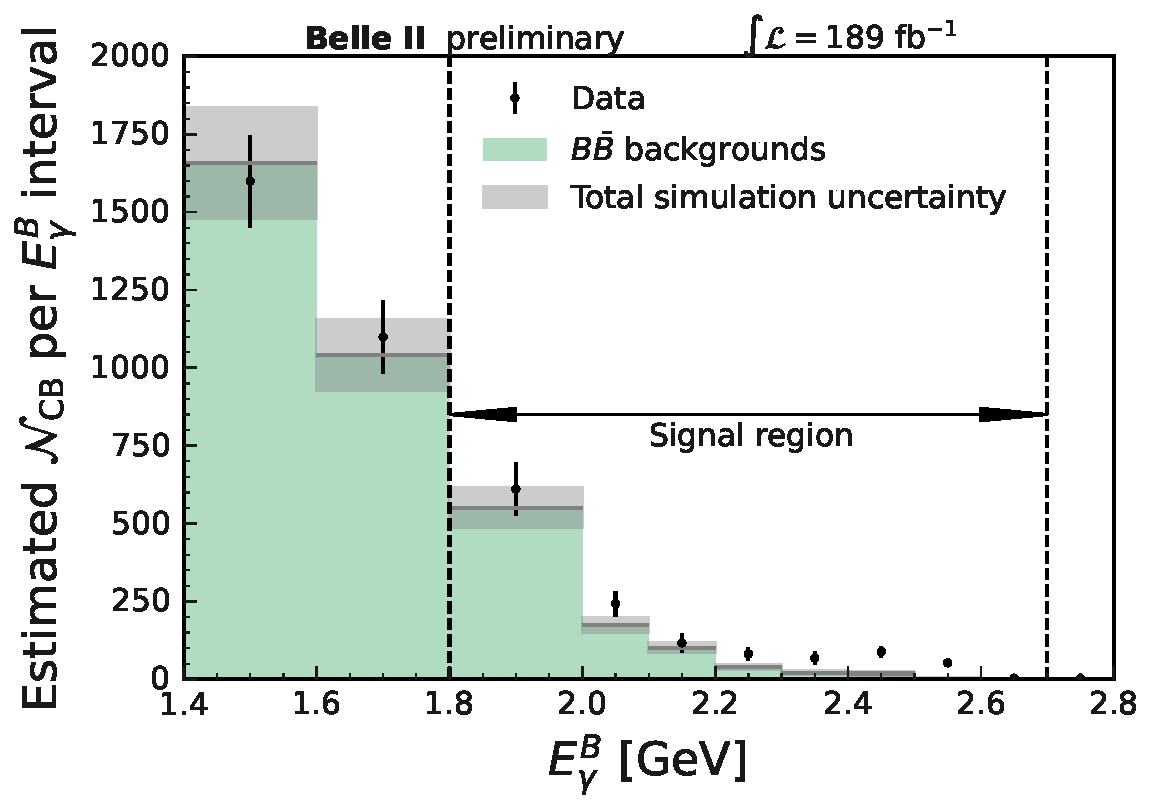
\includegraphics[width=0.45\textwidth]{figures/final_results/background_vs_data_final.pdf}
    }
    \subcaptionbox{\label{fig:final_fit_results_log}}{
        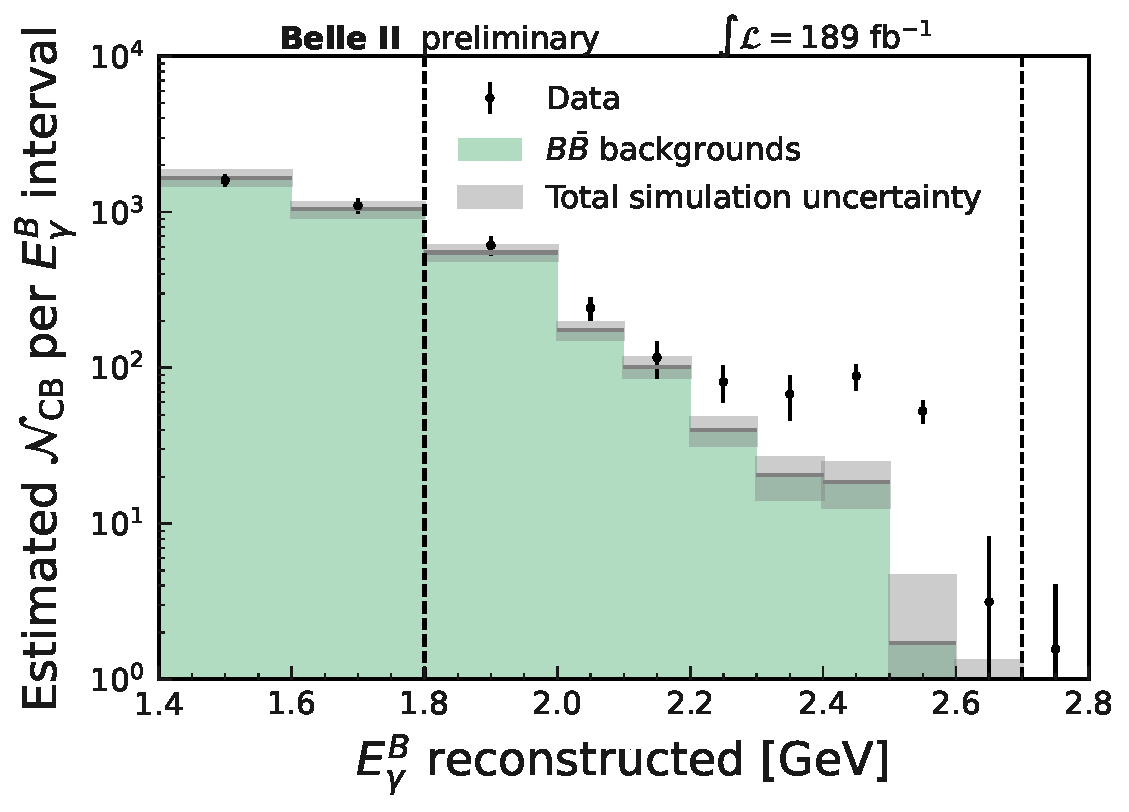
\includegraphics[width=0.45\textwidth]{figures/final_results/background_vs_data_final_log.pdf}
    }
    \caption{\label{fig:final_fit_results}
        The results of fits \Cref{fig:sideband_data_fit,fig:sideband_mc_fit,fig:data_fits_signal,fig:nosignal_fits_signal}.
        All corrections discused in \Cref{tab:correction_table} are applied, 
        and relevant uncertainties from \Cref{tab:background_uncertainties,tab:fit_uncertainties} are included.
        \Cref{fig:final_fit_results_lin} show the results in a linear, whereas \Cref{fig:final_fit_results_log} in a logarithmic axis.
        The excess seen in Belle~II data is evidence of the presence of \BtoXsdgamma events.
    }
\end{figure}

\subsection{Remaining-\texorpdfstring{\BB}{BB} background subtraction results}\label{sec:background_subtraction_results}

The excess that is observed in Belle~II data fits over background-only Belle~II simulation fits is attributed to the presence of \BtoXsdgamma events.
Following the background subtraction strategy shown in \Cref{sec:background_subtraction,sec:background_subtraction_validation_mc},
the remaining good tag-\B meson backgrounds are subtracted.
Simply put, this corresponds to the subtraction of the filled (green) histogram from data points in \Cref{fig:final_fit_results}.
Within uncertainties, the resulting difference can only be accounted by photons that originate in \BtoXsdgamma decays.
The background-subtracted photon energy spectrum is shown in.